\documentclass[]{article}
\usepackage{graphicx}
\usepackage[svgnames]{xcolor} 
\usepackage{fancyhdr}
\usepackage{fancyvrb}
\usepackage{forest}
\usepackage{tocloft}
\usepackage[hidelinks]{hyperref}
\usepackage{enumitem}
\usepackage[many]{tcolorbox}
\usepackage{listings }
\usepackage[a4paper, total={6in, 8in} , top = 2cm,bottom = 4cm]{geometry}
%\usepackage[a4paper, total={6in, 8in}]{geometry}
\usepackage{afterpage}
\usepackage{amssymb}
\usepackage{pdflscape}
\usepackage{textcomp}
\usepackage{xecolor}
\usepackage{rotating}
\usepackage[Kashida]{xepersian}
\usepackage[T1]{fontenc}
\usepackage{tikz}
\usepackage[utf8]{inputenc}
\usepackage{PTSerif} 
\usepackage{seqsplit}
\usepackage{changepage}


\usepackage{listings}
\usepackage{xcolor}
\usepackage{sectsty}

\setcounter{secnumdepth}{0}
 
\definecolor{codegreen}{rgb}{0,0.6,0}
\definecolor{codegray}{rgb}{0.5,0.5,0.5}
\definecolor{codepurple}{rgb}{0.58,0,0.82}
\definecolor{backcolour}{rgb}{0.95,0.95,0.92}
\definecolor{blanchedalmond}{rgb}{1.0, 0.92, 0.8}
\definecolor{brilliantlavender}{rgb}{0.96, 0.73, 1.0}
 
\NewDocumentCommand{\codeword}{v}{
\texttt{\textcolor{blue}{#1}}
}
\lstset{language=java,keywordstyle={\bfseries \color{blue}}}

\lstdefinestyle{mystyle}{
    backgroundcolor=\color{backcolour},   
    commentstyle=\color{codegreen},
    keywordstyle=\color{magenta},
    numberstyle=\tiny\color{codegray},
    stringstyle=\color{codepurple},
    basicstyle=\ttfamily\normalsize,
    breakatwhitespace=false,         
    breaklines=true,                 
    captionpos=b,                    
    keepspaces=true,                 
    numbers=left,                    
    numbersep=5pt,                  
    showspaces=false,                
    showstringspaces=false,
    showtabs=false,                  
    tabsize=2
}

\lstset{style=mystyle}

 \settextfont[BoldFont={XB Zar bold.ttf}]{XB Zar.ttf}


\setlatintextfont[Scale=1.0,
 BoldFont={LiberationSerif-Bold.ttf}, 
 ItalicFont={LiberationSerif-Italic.ttf}]{LiberationSerif-Regular.ttf}





\newcommand{\inputsample}[1]{
    ~\\
    \textbf{ورودی نمونه}
    ~\\
    \begin{tcolorbox}[breakable,boxrule=0pt]
        \begin{latin}
            \large{
                #1
            }
        \end{latin}
    \end{tcolorbox}
}

\newcommand{\outputsample}[1]{
    ~\\
    \textbf{خروجی نمونه}

    \begin{tcolorbox}[breakable,boxrule=0pt]
        \begin{latin}
            \large{
                #1
            }
        \end{latin}
    \end{tcolorbox}
}

\newtcolorbox{mybox}[2][]{colback=red!5!white,
colframe=red!75!black,fonttitle=\bfseries,
colbacktitle=red!85!black,enhanced,
attach boxed title to top center={yshift=-2mm},
title=#2,#1}

\newenvironment{changemargin}[2]{%
\begin{list}{}{%
\setlength{\topsep}{0pt}%
\setlength{\leftmargin}{#1}%
\setlength{\rightmargin}{#2}%
\setlength{\listparindent}{\parindent}%
\setlength{\itemindent}{\parindent}%
\setlength{\parsep}{\parskip}%
}%
\item[]}{\end{list}}


\definecolor{foldercolor}{RGB}{124,166,198}
\definecolor{sectionColor}{HTML}{ff5e0e}
\definecolor{subsectionColor}{HTML}{008575}

\definecolor{listColor}{HTML}{00d3b9}

\definecolor{umlrelcolor}{HTML}{3c78d8}

\definecolor{subsubsectionColor}{HTML}{3c78d8}

\defpersianfont\authorFont[Scale=0.9]{XB Zar bold.ttf}

\defpersianfont\titr[Scale=1.5]{Lalezar-Regular.ttf}

\defpersianfont\fehrest[Scale=1.2]{Lalezar-Regular.ttf}

\defpersianfont\fehrestTitle[Scale=3.0]{Lalezar-Regular.ttf}

\defpersianfont\fehrestContent[Scale=1.2]{XB Zar bold.ttf}


\sectionfont{\color{sectionColor}}  % sets colour of sections
\subsectionfont{\color{subsectionColor}}  % sets colour of sections
\subsubsectionfont{\color{subsubsectionColor}}


\renewcommand{\labelitemii}{$\circ$}


\renewcommand{\baselinestretch}{1.1}


\renewcommand{\contentsname}{فهرست}

\renewcommand{\cfttoctitlefont}{\fehrestTitle}


\renewcommand\cftsecfont{\color{sectionColor}\fehrestContent\selectfont}
\renewcommand\cftsubsecfont{\color{subsectionColor}\fehrestContent\selectfont}
\renewcommand\cftsubsubsecfont{\color{subsubsectionColor}\fehrestContent\selectfont}
%\renewcommand{\cftsecpagefont}{\color{sectionColor}}

\setlength{\parskip}{1.2pt}

\begin{document}


%%% title pages
\begin{titlepage}
\begin{center}

\textbf{ \Huge{به نام خدا} }
        
\vspace{0.2cm}


\includegraphics[width=0.4\textwidth]{sharif1.png}\\
\vspace{0.2cm}
\textbf{ \Huge{\emph درس برنامه‌سازی پیشرفته} }\\
\vspace{0.25cm}
\textbf{ \Large{ فاز دوم پروژه} }
\vspace{0.2cm}
       
 
      \large \textbf{دانشکده مهندسی کامپیوتر}\\\vspace{0.1cm}
    \large   دانشگاه صنعتی شریف\\\vspace{0.2cm}
       \large   ﻧﯿﻢ سال دوم 00-99 \\\vspace{0.10cm}
      \noindent\rule[1ex]{\linewidth}{1pt}
استاد:\\
    \textbf{{دکتر محمدامین فضلی}}



    \vspace{0.20cm}

   مهلت ارسال:\\
    \textbf{{4 تیرماه ۱۴۰۰}}
    \textbf{{ساعت ۲۳:۵۹:۵۹}}

    \vspace{0.10cm}
مسئول پروژه:\\
    \textbf{\authorFont{امیرمهدی نامجو}}
    
        \vspace{0.10cm}
مسئول فاز دوم:\\
    \textbf{\authorFont{فاطمه خاشعی}}
    
        \vspace{0.10cm}
طراحان فاز دوم:\\
    \textbf{\authorFont{نازنین آذریان، پویا اسمعیلی،‌ علی حاتمی، علیرضا هنرور}}
    
        \vspace{0.05cm}
مسئولین تنظیم مستند:\\
    \textbf{\authorFont{پارسا محمدیان و سروش جهان‌زاد}}
    

\end{center}
\end{titlepage}
%%% title pages


%%% header of pages
\newpage
\pagestyle{fancy}
\fancyhf{}
\fancyfoot{}
\cfoot{\thepage}
\lhead{فاز دوم}
\rhead{
\includegraphics[width=0.1\textwidth]{sharif.png}\\
دانشکده مهندسی کامپیوتر
}
\chead{پروژه برنامه‌سازی پیشرفته}
%%% header of pages
\renewcommand{\headrulewidth}{2pt}

\KashidaOff



\tableofcontents

\newpage

 \Large \textbf{\\\\
}


\section*{{\titr نکات قابل توجه}}
\addcontentsline{toc}{section}{{\fehrestContent نکات قابل توجه}}
\begin{itemize}
\item
پس از اتمام این فاز، در گیت خود یک تگ با ورژن \lr{"v2.0.0"} بزنید. در روز تحویل حضوری این tag بررسی خواهد شد و کدهای پس از آن نمره‌ای نخواهد گرفت. برای اطلاعات بیش‌تر در مورد شیوه ورژن‌گذاری، می‌توانید به
 \href{https://semver.org/}{\textcolor{blue}{\underline{این لینک}}}
 مراجعه کنید. البته برای این پروژه صرفا رعایت کردن همان ورژن گفته شده کافیست، اما خوب‌ است که با منطق ورژن‌بندی هم آشنا بشوید.

\item
در روز تحویل حضوری مشارکت تمام اعضای تیم در پروژه بررسی خواهد‌ شد و در صورت عدم مشارکت بعضی از اعضا، نمره‌ی ایشان برای آن فاز پروژه "صفر" لحاظ می‌گردد. مشارکت، با توجه به commit های افراد تیم در مخزن گیت‌هاب پروژه بررسی می‌شود.

\item
در هر فاز می‌توانید سه روز تاخیر به ازای کسر نمره داشته‌ باشید که به ازای هر روز آن، ۱۰ درصد از نمرهٔ آن فاز را از دست خواهید‌ داد. در مجموع سه‌فاز پروژه، سه روز تاخیر نیز بخشیده خواهد‌ شد.

\item
به ازای هر ساعتی که پروژه را زودتر تحویل دهید، ۱۵ دقیقه به مهلت تاخیر بدون کسر نمره شما اضافه خواهد‌ شد. این مقدار حداکثر یک روز خواهد‌ بود که در صورت ارسال ۴ روز زودتر از ددلاین به شما تعلق خواهد گرفت. \textbf{بنابراین ددلاین‌های پروژه تحت هیچ شرایطی تمدید نخواهد‌ شد.} توصیه می‌شود با برنامه‌ریزی مناسب به ددلاین‌های درس پایبند باشید.

\item
در صورت کشف تقلب از هریک از تیم‌ها، برای بار اول منفی نمرهٔ آن فاز برای آن تیم ثبت می‌شود و برای بار دوم، نمرهٔ منفی کل پروژه برای تیم لحاظ خواهد‌ شد که معادل مردود شدن در درس است.


\end{itemize}

\newpage

\section*{{\titr مقدمه}}
\addcontentsline{toc}{section}{{\fehrestContent مقدمه}}

\section*{{\titr نکات}}
\addcontentsline{toc}{section}{{\fehrestContent نکات}}
در طراحی گرافیک خود نکات زیر را در نظر داشته باشید:

\begin{itemize}
    \item در طراحی بازی یکی از نکاتی که باید در نظر داشت \lr{user friendly} بودن محیط بازی است به این معنی که در استفاده از آن ابهامی وجود نداشته باشد و به سادگی بتوان فهمید که هر عنصر بیانگر چه چیزی است یکی از را‌ه‌های رسیدن به آن حذف هرگونه عنصر اضافی و همچنین استفاده از \lr{sprite} های مناسب برای هر قسمت است.
    \item استفاده از فونت و رنگ مناسب در محیط بازی اهمیت دارد به این صورت که نوشته‌ها باید کاملا واضح و خوانا باشند. برای مثال استفاده از رنگ متنی که تفاوت زیادی با رنگ \lr{background} ندارد خوانایی متن را کاهش می‌دهد.
    \item در هر بخش بعضا یک چینش برای آن بخش پیشنهاد داده شده است اما هیچ اجباری برای طراحی صفحه به آن صورت نیست و می‌توانید خواسته‌های هر بخش را هر طور که مایلید پیاده‌سازی کنید اما دقت کنید که تمام قابلیت‌های خواسته شده باید در پیا‌ده‌سازی شما وجود داشته باشد.
\end{itemize}

\section*{{\titr جزئیات}}
\addcontentsline{toc}{section}{{\fehrestContent جزئیات}}

\subsection*{{\titr منوها}}
\addcontentsline{toc}{subsection}{{\fehrestContent منوها}}

\begin{itemize}
    \item تمامی منو‌های پیاده‌سازی شده باید از منوی‌ اصلی در دسترس باشند و همچنین امکان برگشت از آنها به منوی اصلی باید وجود داشته باشد.
    \item تمامی‌ منو‌ها باید دارای \lr{background} مناسب باشند.
    \item اگر در حین انجام هر عملیاتی به خطا برخوردید باید این خطا به طور مناسب نشان داده شود.خطا را با توجه به نوع آن می‌توانید در متنی زیر دکمه‌ی انجام عملیات،  زیر \lr{element} ورودی کاربر و یا در قالب  یک \lr{pop up} را نشان دهید.
    \item \textbf{امتیازی}: تغییر شکل نشان‌گر موس در بازی نمره امتیازی دارد. مثلا در هنگام حمله به کارت‌ها شکل آن به صورت دیگری در بیاید و یا در صورتی که روی گزینه غیرفعالی قرار گرفت به شکل ضربدر در بیاید. پیاده‌سازی این مورد برای یک مورد برای گرفتن نمره امتیازی آن کافی است. 
\end{itemize}


\subsection*{{\titr ثبت‌نام و ورود}}
\addcontentsline{toc}{subsection}{{\fehrestContent ثبت‌نام و ورود}}
\begin{itemize}
	\item \lr{\textbf{Register}}:
	سه ورودی نام کاربری، نام مستعار و رمز از کاربر گرفته شده و در صورت عدم وجود خطا حساب کاربری ساخته می‌شود، پس از ساخته شدن حساب کاربری باید کاربر را از این موضوع مطلع کنیم برای مثال می‌توانید در زیر دکمه‌ی ثبت‌نام با رنگ سبز عبارت زیر را نمایش دهید.
	
	
	\begin{mybox}[colback=yellow]{پیغام به کاربر}
		\begin{latin}	
			User created successfully.
		\end{latin}
	\end{mybox}
	
	\item
	حساب کاربری باید یک عکس پروفایل داشته باشد، با ساختن حساب کاربری باید از یک سری عکس‌های از پیش تعیین شده به صورت رندوم یکی را انتخاب کرده و به عنوان عکس پروفایل حساب کاربری قرار دهیم.
	\item \lr{\textbf{Login}}:
	با دریافت نام کاربری و رمز از کاربر در صورت اعتبارسنجی، باید عملیات ورود انجام شده و از این منو به منوی اصلی بازی منتقل شویم.
\end{itemize}


\subsection*{{\titr منو اصلی}}
\addcontentsline{toc}{subsection}{{\fehrestContent منو اصلی}}

\begin{itemize}
    \item
     منوی اصلی برنامه ما است. در این منو باید امکان ورود به منو‌های دیگر وجود داشته باشد.
    \item
     \lr{\textbf{Logout}}: دکمه‌ای تحت این عنوان وجود داشته باشد تا با کلیک روی آن از حساب کاربری خارج شده و به منوی \lr{Register/Login} منتقل شویم.
\end{itemize}

\subsection*{{\titr دسته کارت}}
\addcontentsline{toc}{subsection}{{\fehrestContent دسته کارت}}
\begin{itemize}
    \item \textbf{نمایش لیست دک‌های کاربر}: در این صفحه همه دک های کاربر و تعداد کارت‌های داخل آن‌ها نشان داده می‌شود. دک فعال باید در این صفحه مشخص باشد.
    \item \textbf{حذف یا ویرایش یک دک}:
     برای هر دک باید امکان حذف یا ویرایش آن وجود داشته باشد. با کلیک روی دکمه‌ی حذف دک حذف می‌شود و با کلیک روی دکمه ویرایش وارد صفحه مربوط به آن دک می شویم.
     
    \item \textbf{گزینه ساخت دک جدید}:
     در این صفحه باید دکمه ای برا ایجاد دک جدید وجود داشته که در صورت انتخاب آن نام دک جدید را از کاربر بگیرد و در صورت معتبر بودن نام  یک دک ساخته شود و کاربر پیام زیر را مشاهده کند:
     
     \begin{mybox}[colback=yellow]{پیغام به کاربر}
     	\begin{latin}	
     		Deck created successfully
     	\end{latin}
     \end{mybox}
 
    \item \textbf{انتخاب یک دک به عنوان دک فعال}:
     کاربر باید بتواند یکی از دک‌های خود را به عنوان دک فعال انتخاب کند و یا دک فعالش را تغییر دهد می‌توانید در قالب یک دکمه در کنار حذف و ویرایش یک دک این قابلیت را داشته باشید یا در صفحه دک بتوانید آن را به عنوان یک دک فعال انتخاب کنید.
     
    \item \textbf{جزئیات دک}:
     با کلیک روی دک باید جزئیات آن نشان داده شود. برای این کار می‌توانید یک صفحه جزئیات دک داشته باشید. برای هر دک نام آن و کارت‌های آن نمایش داده می‌شود. کارت‌های دک اصلی و دک فرعی (\lr{Side Deck}) باید مجزا نشان داده شوند. همچنین کاربر باید بتواند کارت یک دک را حذف کند یا به دک کارت اضافه کند.
    \item 
    برای اضافه کردن کارت به دک پس از کلیک روی دکمه مورد نظر باید امکان نمایش همه کارت های کاربر وجود داشته باشد تا اگر خواست بتواند کارتی را در صورت امکان به دک خود اضافه کند.س

     
    \item \textbf{نمایش کارت‌های داخل دک با نگه داشتن موس روی آن (امتیازی)}:
    اگر با نگه داشتن موس روی هر دک کارت‌های آن دک را نمایش دهید به شما نمره امتیازی تعلق می‌گیرد.    
\end{itemize}
\begin{center}
	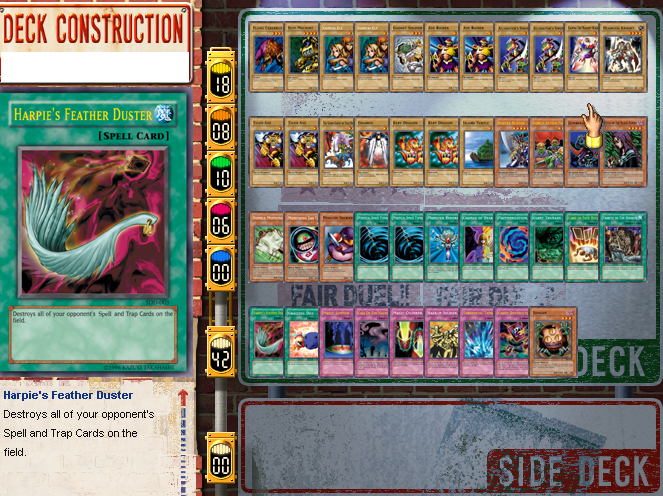
\includegraphics[width = 0.75 \textwidth]{images/1.png}
	
\end{center}

\subsection*{{\titr فروشگاه}}
\addcontentsline{toc}{subsection}{{\fehrestContent فروشگاه}}

\begin{itemize}
    \item \textbf{نمایش لیست کارت‌ها}:
     باید عکس هر کارت که شامل مشخصات هر‌کدام، که بستگی به نوع کارت دارد، نشان داده شود.
     
    \item \textbf{خرید کارت}:
     در کنار هر کارت باید گزینه خرید وجود داشته باشد که در صورت کلیک روی آن قیمت کارت از حساب کابر کم شده و کارت به لیست کارت های کاربر اضافه شود. بعد از نهایی شدن خرید کارت و اضافه شدن آن به لیست کارت‌های کاربر، باید پیام زیر نمایش داده شود:
     
     
    
     
     \begin{mybox}[colback=yellow]{پیغام به کاربر}
     	\begin{latin}	
     		Card added successfully
     	\end{latin}
     \end{mybox}
     
    \item \textbf{تعداد موجود از کارت}:
     در صورتی که کاربر یک یا چند بار یک کارت را خریده باشد یا به عبارت دیگر موجودی کارت صفر نباشد، تعداد موجود برای هر کارت خریداری شده نشان داده شود.
     
    \item \textbf{امتیازی}: در صورتی که قیمت کارتی از موجودی کاربر بیشتر بود دکمه‌ی \lr{buy} کارت غیر‌فعال باشد.
\end{itemize}




\subsection*{{\titr جدول امتیازات}}
\addcontentsline{toc}{subsection}{{\fehrestContent جدول امتیازات}}

\begin{itemize}
    \item \lr{\textbf{Scoreboard}}: 
     لیست ۲۰ کاربری که امتیازشان از بقیه بیشتر است نشان داده شود که در هر سطر، شماره سطر،  نام مستعار کاربر و امتیاز او وجود دارد. اگر کاربر فعلی در آن لیست وجود دارد رنگ سطر او با بقیه فرق داشته باشد.
\end{itemize}


\subsection*{{\titr پروفایل}}
\addcontentsline{toc}{subsection}{{\fehrestContent پروفایل}}
\begin{itemize}
    \item \textbf{عکس پروفایل}:
     برای هر کاربر یک عکس پروفایل وجود دارد که با ساخت اکانت یکی از عکس‌های \lr{default} برای پروفایل کاربر انتخاب می‌شود.
    \item \textbf{نام کاربری}:
     نام کاربری کاربر باید در این منو در دسترس باشد اما قابلیت تغییر آن وجود ندارد.
    \item \textbf{نام مستعار}:
     نام مستعار کاربر باید نشان داده شده و کاربر می‌تواند نام مستعار خود را تغییر دهد.
    \item \textbf{تغییر رمز عبور}:
     برای تغییر رمز عبور باید رمز قبلی و رمز جدید را به عنوان ورودی از کاربر گرفته و در صورت اعتبارسنجی عملیات انجام شود.
     
    \item \textbf{امتیازی}: کاربر بتواند با آپلود عکس جدید، عکس پروفایل‌ خود را عوض کند. با توجه به این که در این فاز مفهوم شبکه وجود ندارد، آپلود به این معناست که عکسی از روی سیستم شما انتخاب شده و به داده‌های برنامه اضافه بشود و بعدا بتوان از آن استفاده کرد.
\end{itemize}

\subsection*{{\titr ایمپورت و اکسپورت}}
\addcontentsline{toc}{subsection}{{\fehrestContent ایمپورت و اکسپورت}}
\begin{itemize}
    \item \textbf{عملیات \lr{import}}:
     می‌توانید یک جایگاه آپلود فایل قرار داده تا با \lr{drag and drop} فایل‌ها و یا فشردن دکمه و انتخاب فایل عملیات \lr{import} انجام شود و پس از انجام عملیات مشخصات کارت \lr{import} شده نمایش داده شود.
    \item نحوه نمایش مشخصات کارت دلخواه است برای مثال می‌توانید یک جایگاه برای نمایش کارت‌ها در نظر گرفته و با انجام عملیات \lr{import} مشخصات کارت را در آنجا نمایش دهید و یا اینکه پس از \lr{import} در قالب یک پنجره \lr{popup} مشخصات کارت مورد نظر را نمایش دهید.
    \item \textbf{عملیات \lr{export}}: با فشردن دکمه \lr{Export} کارت‌های قابل انتخاب نمایش‌داده می‌شوند و با انتخاب یک کارت، همانند فاز یک آن را در فایلی \lr{Export} کنید.
    \item \textbf{امتیازی}: بتوانید فایل با حداقل دو پسوند‌ متفاوت (برای مثال \lr{json} و \lr{csv}) را مدیریت کنید.
\end{itemize}

\subsection*{{\titr بازی}}
\addcontentsline{toc}{subsection}{{\fehrestContent بازی}}
زمین بازی و فرایندهایی که درون آن اتفاق ‌می‌افتد یکی از بخش‌های اساسی فاز دوم خواهد بود. این بخش نیز مانند بخش‌های دیگر شامل جزئیاتی خواهد بود که باید آن را پیاده‌سازی کنید.  در ادامه به جزئیاتی که در بازی هستند می‌پردازیم. از شما انتظار می‌رود تا بازی که در فاز اول طراحی شده بوده و با دستورات کنسول کنترل می‌شد به صورت گرافیکی دربیاید (مواردی که جزء دستورات در فاز اول بوده است ولی بعدتر از آنها صحبتی نشده است هم باید پیاده‌سازی شود اما نحوه طراحی و پیاده‌سازی آن به خود شما سپرده شده است و می‌توانید از خلاقیت خود در پیاده‌سازی آنها استفاده کنید)‌:

\begin{itemize}
    \item \textbf{زمین بازی}:
     زمین‌بازی و کارت‌های درون آن باید در صفحه حضور داشته باشند. هر کاربر باید کارت‌های خود را ببیند و عملیات‌های مربوط به آن را انجام دهد (کمی جلوتر درباره آن توضیح داده خواهد شد).
    \item \textbf{مشخصات دوئلیست‌ها}:
     در بازی صفحه بازی باید آواتار، \lr{LP} (جان)، نام‌کاربری و نام مستعار هر دو دوئلیست باید در صفحه وجود داشته باشد.
    \item \textbf{تغییر فازها}:
     باید قسمتی برای تغییر فازها برای کاربر وجود داشته باشد تا اتمام دورش را اعلام کند.
     
    \item \textbf{مشخصات کارت‌ها}:
     باید قسمتی وجود داشته باشد که بعد از انتخاب هر کارتی که ماهیت آن برای کاربر فعال (بازیکنی که باید حرکت خود را انجام دهد) مشخص است (شامل کارت‌های به روی حریف و تمام کارت‌های خودش که درون زمین یا در دستش است) مشخصات آن شامل نوع آن، بخش‌های اختصاصی مربوط به نوع آن (برای مثال قدرت حمله و دفاع در هیولاها)، توضیحات اضافه و … نمایش داده شوند.
    \item \textbf{تصویر زمینه}:
     در پس‌زمینه صفحه بازی باید از یک تصویر استفاده شده باشد.
    \item \textbf{امتیازی}:برای کارت‌های خاصی (مثلا کارت‌های \lr{Field}) این تصویر زمینه مطابق با کارتی که در زمین فعال است تغییر کند.
    
    \item \textbf{وقفه}: در حین بازی باید امکان وقفه بین بازی وجود داشته باشد. چیزی مثل یک منو \lr{Pause} که در آن امکان خروج از بازی، تغییر تنظیمات مربوط به بازی و … در آن وجود داشته باشد.
    \item \textbf{حمله}: در فاز نبرد (\lr{Battle Phase}) که امکان حمله برای هیولاها فراهم می‌شود، امکان حمله به کارت ها از طریق رابط‌های گرافیکی مثل انتخاب کارت مهاجم و کارت هدف به وسیله کلیک موس و یا درگ‌اند‌دراپ (امتیازی) فراهم شود.
    
    \item \textbf{نمایش گورستان کارت‌ها}: در حین بازی باید امکان نمایش گورستان برای بازیکن‌ها وجود داشته باشد و انتظار می‌رود تا در هنگام نمایش گورستان کارت‌ها به همراه عکس آنها به بازیکن نمایش داده شود، در صفحه اصلی بازی لازم نیست همواره گورستان نمایش داده شود، می‌توان یک دکمه برای آن قرار داد و در صورت نیاز با کلیک روی دکمه جزئیات گورستان کارت‌ها نشان داده شود.
    
    
    \item \textbf{انتخاب کارت برای فرایندهای خاص}: برخی از فرایندهای بازی نیاز به انتخاب کارتهایی از زمین بازی دارد. انتظار می‌رود تا تمام انتخاب‌های ممکن به بازیکن نشان داده شود تا بتواند کارت(های) مورد نظرش را انتخاب کند و فرآیند بر روی آنها انجام شود.
    
    
    \item \textbf{انیمیشن کارت‌ها}: انتظار می‌رود تا تغییراتی که در صفحه بازی انجام می‌شود (مثل کشیدن کارت از دک به دست، رفتن یک کارت از زمین به گورستان، حمله کارت‌ها و … ) همراه با پویانمایی و حرکاتی نرم و چشم‌نواز (!) باشند. پیاده سازی یک مورد پویانمایی اجباری خواهد بود اما موارد بیشتر با توجه به داک نمرات و موارد موجود در آن امتیازی خواهد بود.
    
    
    \item \textbf{محرمانه بودن کارت‌های حریف}:
     موردی که باید به آن توجه کافی را داشته باشید این است که در فاز بعد قرار است تا دو بازیکن به صورت مستقل از هم و برای مثال با دو رایانه جدای از هم بازی را انجام دهند. بدیهی است که یک بازیکن کارت‌هایی که در دست بازیکن دیگر است و یا کارت‌هایی که به پشت در زمین حریف‌ هستند را نباید ببینید. همینطور انجام عملیات برای بازیکنی که نوبت او نیست محدود است و نمی‌تواند حرکتی انجام دهد. \\
    به همین منظور در این فاز هم باید شرایط مشابهی را در پیاده سازی خود در نظر بگیرید تا در پیاده‌سازی فاز بعد نیاز به تغییرات اساسی در برنامه خود بی‌نیاز شوید. انتظار می‌رود تا محرمانه بودن کارت‌های حریف در هر نوبت را رعایت کنید اما شیوه  پیاده سازی شما بسته به نوع طراحی که برای بازی دارید می‌توان متغیر باشد. در ادامه دو شیوه برای پیاده سازی این قابلیت پیشنهاد می‌شود:
    \begin{itemize}
        \item حالتی که هر دو بازیکن در یک پنجره (\lr{Window}) در حال بازی کردن باشند:‌ مخفی کردن و نمایان کردن کارت ها در هر دور، یعنی زمانی که نوبت‌ها تغییر می‌کند، کارت‌هایی که باید مخفی شوند در سمت دیگر صفحه به پشت می‌شوند و کارت‌هایی که از نوبت قبل برای بازیکن قبل قابل نمایش نبوده اند نیز به حالت رو در بیایند تا برای بازیکنی که نوبت آن است قابل مشاهده باشند. این تغییرات می‌تواند همراه با یک چرخش صفحه هم همراه باشد.
        \item حالتی که برای هر بازیکن یک پنجره جداگانه در نظر گرفته شود: می‌توانید پیاده‌سازیتان را (که به چیزی که در فاز بعد مورد نیاز است نزدیکتر است) با استفاده از دو پنجره انجام دهید به این صورت که زمانی که یک دوئل آغاز می‌شود دو پنجره بسازید که هر دو با یک کلاس مشترک که مسئول هماهنگی این دو پنجره است در ارتباط باشند. هر پنجره مربوط به یک بازیکن است. بدیهی است که رابط کاربری در هر دوپنجره کاملا مشابه خواهد بود با این تفاوت که انگار زمین بازی چرخیده و کارت‌های حریف در سمت دیگر قرار خواهد داشت. 
    \end{itemize}
    \item \textbf{چت باکس}: در فاز بعد به برنامه شما یک \lr{Chatbox} به برنامه اضافه خواهد شد. این قسمت کاملا مربوط به فاز بعد خواهد بود اما پیشنهاد می‌شود تا تدابیر (!) لازم را بیندیشید (مثلا محل مناسبی برای آن پیدا کنید) تا در فاز بعد به مشکلی برنخورید.
    \item \textbf{تقلب}:
    ‌ انتظار می‌رود در بازی امکان تقلب کردن (چه به منظور رفع عیب برنامه و یا سخت‌تر کردن بازی حریف) وجود داشته باشد. می‌توانید این تقلب را در قالب یک کنسول \lr{transparent} روی بازی داشته باشید که زمانی که دکمه‌های \lr{ctrl+shift+c} فشرده شدند کنسول ظاهر شود و دستورات مربوط به تقلب فاز قبل را وارد کنید.
    
    \item \textbf{انیمیشن \lr{Sprite}}:
     در صفحه بازی حداقل برای یک عملیات (مثلا نابود شدن یک هیولا) باید از انیمیشن‌های \lr{Sprite} استفاده کنید. برای این بخش می‌توانید از Asset هایی که در اختیارتان قرار خواهد گرفت استفاده کنید.
     
     
    \item \textbf{موسیقی بازی}: بازی شما باید یک موسیقی متناسب داشته باشد. ( امتیازی ) 
    \begin{itemize}
        \item می‌توانید افکت‌های صدا در شرایطی خاص که در بازی به وجود می‌آید پخش کنید، برای مثال زمانی که یک کارت \lr{Field} فعال است و یا مقدار کمی از جان حریف باقی‌مانده است. ( امتیازی‌ )
    \end{itemize}
    \item \textbf{پیغام برد یا باخت}: در انتهای بازی باید یک دیالوگ مبتنی بر برد یا باخت فرد و امتیاز او به او نشان داده شود و گزینه‌هایی مثل بازگشت به صفحه اصلی، انجام دوباره بازی و و موارد مشابه دیگر بسته به صلاحدید خودتان وجود داشته باشد.
    \item \textbf{سکه/سنگ، کاغذ، قیچی}:
    
     در ابتدای بازی باید یک صفحه برای تعیین شروع‌کننده دوئل وجود داشته باشد که یا سکه خواهد بود و یا سنگ‌، کاغذ، قیچی. این که براساس کدام یک جلو بروید،‌ به خودتان بستگی دارد. ( \lr{Asset} های مربوط به هر دو در اختیارتان قرار خواهد گرفت)
     
     
    \item \textbf{کم شدن از جان}: بایستی برای کم شدن جان حریف انیمیشنی در نظر بگیرید. برای مثال می‌توانید کاری کنید که با کم شدن از جان حریف به تدریج رنگ نوشته آن از سبز به سمت قرمز تغییر رنگ دهد. حتی می‌توانید برای جان یک \lr{Bar} در نظر بگیرید.
\end{itemize}
برای الهام گرفتن در طراحی می‌توانید از بازی \lr{Yu-Gi-Oh! Power of Chaos: Joey the Passion} کمک بگیرید.
\begin{center}
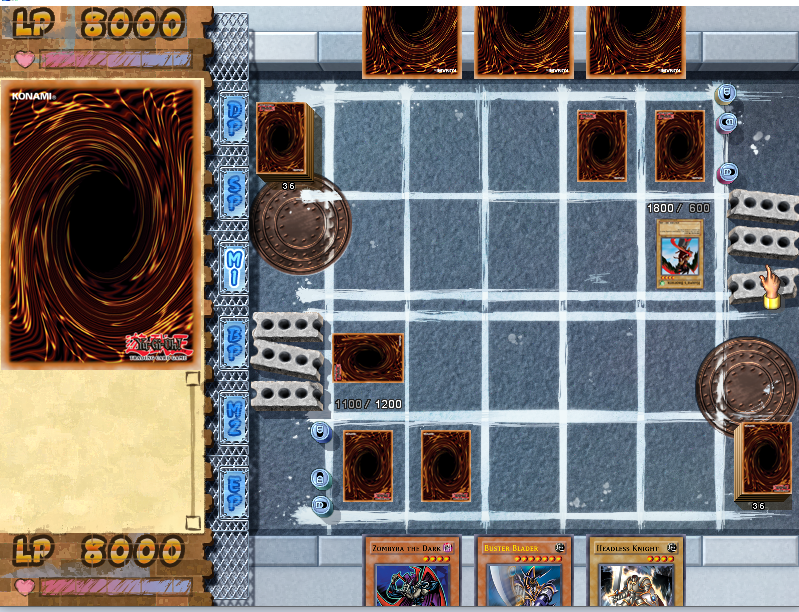
\includegraphics[width = 0.7 \textwidth]{images/2.png}
	
\end{center}


\section*{{\titr سازنده کارت}}
\addcontentsline{toc}{section}{{\fehrestContent سازنده کارت}}

\begin{itemize}
    \item \textbf{اضافه کردن کارت جدید}: باید امکان تعریف کردن کارت جدید را اضافه کنید. برای ساخت یک کارت، مشخصات کارت مانند نوع، سطح، قدرت حمله، قدرت دفاع، توضیحات و … را دریافت کرده و بعد از ساخته شدن کارت باید این کارت در کنار دیگر کارت ها ذخیره شده و امکان خرید آن از فروشگاه وجود داشته باشد.
    \item \textbf{محاسبه ی قیمت کارت جدید}: بعد از وارد کردن مشخصات کارت ، قیمت آن را طبق فرمول دلخواهی بر حسب ویژگی‌های آن محاسبه کنید تا بتوان از فروشگاه این کارت را خرید. همچنین 10 درصد قیمت کارت به عنوان کارمزد از کاربر سازنده ی کارت کسر می شود. \\
    محاسبه ی قیمت در رابط گرافیکی باید همزمان با وارد کردن مشخصات باشد؛ بنابراین با هر تغییر در مشخصات کارت، باید بلافاصله قیمت جدید کارت محاسبه شده و نمایش داده شود.
    \item \textbf{نحوه ی پیاده سازی}: قابلیت ایجاد کارت می‌تواند در هر یک از روابط کاربری شما وجود داشته باشد و انتخاب این مورد به عهده‌ی خود شما است. در حالت گرافیکی می توانید یک تصویر پیش فرض برای همه ی کارت های جدید استفاده کنید. 
    \item \textbf{افکت‌های کارت جدید}: 
    بعضی از کارت های از پیش تعریف شده افکت ‌هاییدارند. در بازی شما باید بتوان ویژگی کارت را از لیست افکت‌های کارت های قبلی انتخاب کرد. بدین منظور یک لیست از همه ی توضیحاتی که برای کارت ها داریم آماده کنید و کاربر بتواند از این لیست انتخاب کند. توجه کنید که مواردی که در این افکت‌ها جنبه متغیر دارند، نظیر اعداد افزایش یا کاهش دفاع و حمله و یا نوع کارت‌هایی که بر روی آن اثر می گذارند، در این بخش باید قابل تغییر باشند.
    
    \item \textbf{امتیازی}: ترکیب افکت‌های چند کارت برای ساخت کارت جدید.

\end{itemize}

\end{document}







